\section{Planlægning}
Der blev fra projektets start udarbejdet en tidsplan.
Gennem hele forløbet har der sideløbende været fokus på både udvikling og rapport/dokumentations skrivning.
Gruppen ønskede ikke at lave enten udvikling eller rapport. Sideløbende med udvikling af systemet, blev der skrevet dokumentation tilhørende dette område. Der skulle også skrives afsnit til rapporten inden man var færdig med opgaven. \\
Dette har betydet at alt dokumentationen er skrevet mens der blev udviklet det var i frisk erindring.
Herunder på figur \ref{fig:Tidsplan} ses gantt-diagrammet for Rambøll Tilsyn. Ud fra dette kan der ses hvordan der er blevet arbejdet med opgaverne gennem hele projektet.

\begin{figure} [H]
	\begin{center}
		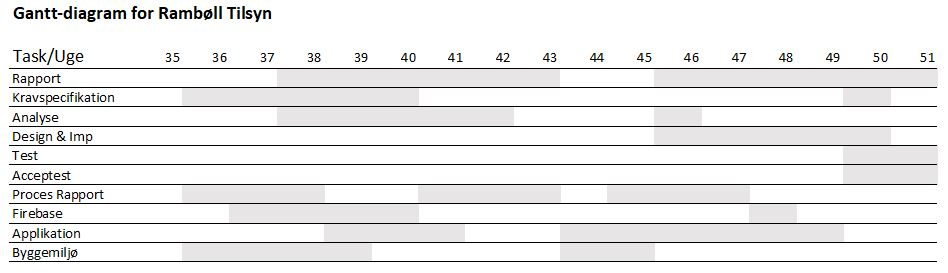
\includegraphics[height=6cm, width=17cm]{Planlaegning/Tidsplan}
	\end{center}
	\caption{Gantt-diagram for projektet.}
	\label{fig:Tidsplan}
\end{figure}

\clearpage

